\documentclass[border=0.2cm]{standalone}
% Required packages and libraries
\usepackage{tikz}
\usetikzlibrary{automata, arrows.meta, positioning}
\begin{document}
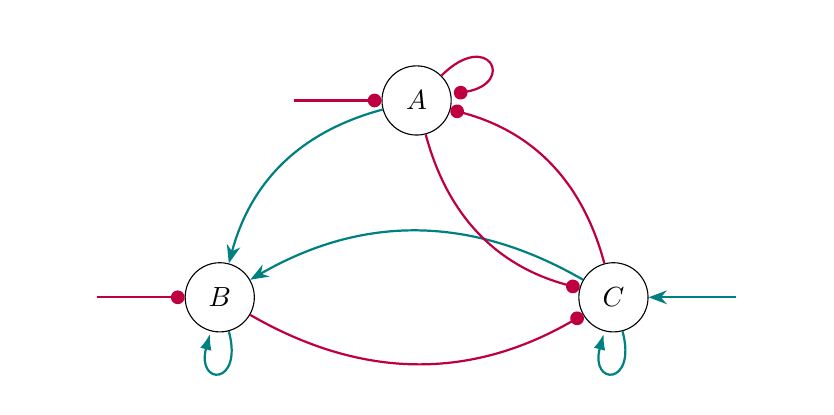
\begin{tikzpicture}
\node (A) [state] at (2.5,2.5) {$A$};
\node (B) [state] at (0,0) {$B$};
\node (C) [state] at (5,0) {$C$};
\node (EA) [state, style={draw=none}] at (0.5,2.5) {};
\node (EB) [state, style={draw=none}] at (-2,0) {};
\node (EC) [state, style={draw=none}] at (7,0) {};
%Activation:
\path [-stealth, thick,every loop/.append style=-{Latex[length=2mm]}]
(A) edge [bend right, -Stealth,color=teal] (B)
(B) edge [loop below,color=teal] ()
(C) edge [bend right, -Stealth,color=teal] (B)
(C) edge [loop below,color=teal] ()
(EC) edge [-Stealth, color=teal] (C)
;
%Repression:
\path [thick,every loop/.append style=-{Latex[length=2mm]},every loop/.append style=-{Circle}]
(A) edge [in =10, out=45, loop,color=purple] (A)
(C) edge [bend right, -Circle,color=purple] (A)
(EA) edge [-Circle,color=purple] (A)
(EB) edge [-Circle,color=purple] (B)
(A) edge [bend right, -Circle,color=purple] (C)
(B) edge [bend right, -Circle,color=purple] (C)
;
\end{tikzpicture}
\end{document}
